\documentclass{article}
\usepackage{graphicx} % Required for inserting images

\usepackage[english, russian]{babel}
\usepackage[T2A]{fontenc}			% кодировка
\usepackage[utf8]{inputenc}			% кодировка исходного текста

\title{\textbf{Лабораторная работа 1.4.2.} \linebreak
ОПРЕДЕЛЕНИЕ УСКОРЕНИЯ СВОБОДНОГО ПАДЕНИЯ ПРИ
ПОМОЩИ ОБОРОТНОГО МАЯТНИКА}
\author{Попова Софья Б04-401}
\date{October 2024}

\begin{document}

\maketitle

\section*{Цель работы}
C помощью оборотного маятника измерить величину ускорения свободного падения

\section*{Оборудование}
Оборотный маятник с двумя подвесными призмами и двумя грузами (чечевицами); электронный счётчик времени и числа колебаний; подставка с острием для определения положения центра масс маятника; закреплённая на стене консоль для подвешивания маятника; металлические линейки, штангенциркуль длиной 1 м.

\section*{Теоретическая часть}
Перед началом работы вспомним несколько понятий: 

\noindent
\textit{Момент инерции} — мера инертности во вращательном движении вокруг оси, подобно тому, как масса тела является мерой его инертности в поступательном движении. 

\noindent
\underline{Теорема Гюйгенса — Штейнера}: момент инерции $J$ тела относительно произвольной неподвижной оси равен сумме момента инерции этого тела $J_C$ относительно параллельной ей оси, проходящей через центр масс тела, и произведения массы тела $m$ на квадрат расстояния $d$ между осями:
\begin{equation}\label{нср}
J=J_C+md^2
\end{equation} 

\noindent
При малых колебаниях период колебаний физического маятника определяется формулой:
\begin{equation}\label{нср}
T=2\pi \sqrt[]{\frac{J}{mgl}}
\end{equation}
где $J$ — момент инерции маятника относительно оси качания, $m$ — масса
маятника, $l$ — расстояние от оси качания до центра масс маятника.

\noindent
\underline{Измерение \textbf{g}}:

\noindent
Пусть $L\equiv\overline{O_1O_2}=l_1+L_2$ - расстояние между двумя "сопряженными" точками подвеса физического маятника. Если соответствующие периоды колебаний равны, $T_1=T_2=T$, то по теореме Гюйнерса $L=L_{np.}$ Тогда находим ускорение свободного падения:
\begin{equation}\label{нср}
g_0 = (2\pi)^2\frac{L}{T^2}
\end{equation} 
Точного совпадения $T_1$ и $T_2$ на опыте добиться невозможно, поэтому получим формулу для определения g, если измеренные переменные незначительно отличаются: $T_1=T$, $T_2 = T+\Delta T$.
\begin{equation}\label{нср}
g = (2\pi)^2\frac{l_1^2-l_2^2}{T_1^2l_1-T_2^2l_2}
\end{equation}
что так же можно переписать как 
\begin{equation}\label{нср}
g = g_0\frac{\lambda -1}{\lambda -\frac{T_2^2}{T_1^2}}
\end{equation}
где $g_0 = (2\pi)^2L/T^2$, a $\lambda = l_1/l_2$.

\noindent
\underline{Оценка погрешностей}:

\noindent
Погрешность определения $g_0$ по формуле (3) равна:
\begin{equation}\label{нср}
\frac{\sigma_{g_0}}{g_0}=\sqrt{(\frac{\sigma_L}{L})^2 + 4(\frac{\sigma_T}{T})^2}
\end{equation}
Это - основная погрешность опыта. Для полной относительной погрешности получим:
\begin{equation}\label{нср}
\frac{\sigma_g}{g}\approx\sqrt{(\frac{\sigma_L}{L})^2 + 4(\frac{\sigma_T}{T})^2 + 8(\beta\frac{\sigma_T}{T})^2 + 8(\beta\frac{\Delta_T}{T}\frac{\sigma_l}{\Delta_l})^2}
\end{equation}
Из этого можно сделать следующие выводы:
\begin{itemize}
    \item При достаточно хорошем совпадении периодов $(\Delta T \ll T)$ погрешность измерения длин $l_1$ и $l_2$ по отдельности, практически не влияет на погрешность конечного результата
    \item Итоговая погрешность неограниченно возрастает при $l_1 \rightarrow l_2$, т.е. когда центр масс маятника оказывается близок к геометрическому центру стержня.
\end{itemize}

\begin{figure}[th!]
    \centering
    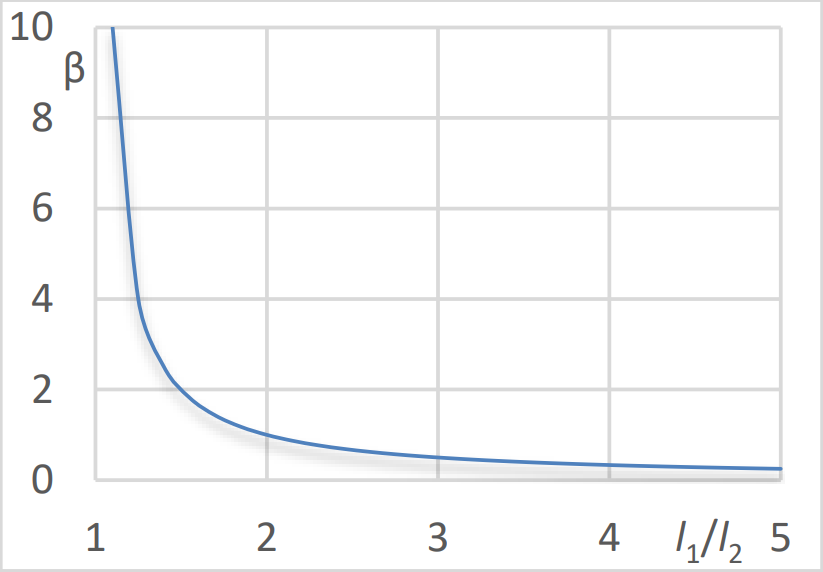
\includegraphics[width=0.5\linewidth]{Screenshot_5.png}
    \caption{Зависимость коэф. $\beta$ от положения центра масс}
    \label{fig:enter-label}
\end{figure}

\section*{Экспериментальная часть}
\underline{1.}

\noindent
Измерим массы отдельных частей маятника, и общую массу 

\noindent
(погрешность: \pm 0,05 г):

\begin{itemize}
    \item Масса стержня: 1018,9 г
    \item Масса 1 груза: 1493,9 г
    \item Масса 2 груза: 1484,3 г
    \item Масса 1 призмы: 59,8 г
    \item Масса 2 призмы: 75,6 г
    \item Масса всего маятника: 4132,2 г
\end{itemize}


\noindent
\underline{2.}

\noindent
Измерим расстояние: 

\noindent
(погрешность: \pm 0,0005 мм):

\noindent
Пусть $L$ - расстояние между призмами, $b_1$ — расстояние от груза Г$_1$ до призмы П$_2$, а $b_2$ — расстояние от груза Г$_2$ до призмы П$_2$. Расположение грузов вычесленно по первой методике из приложения (рассчет и использованием моментов инерции относительно подвеса). Расположение центра масс определено с помощью $\perp$-образной подставки 

\begin{itemize}
    \item L = 60,1 см
    \item $b_1$ = 28 см
    \item $b_2$ = 14,7 см
    \item центр масс - 35 см
\end{itemize}

\noindent
Тогда $l_1=45,2$ см ; $b_2=14,8$ см

\newpage

\noindent
\underline{3.}

\noindent
Проведем серию опытов 

\noindent
Для n = 20 колебаний: 


\begin{table}[th!]
    \centering
    \begin{tabular}{|c|c|c|}
    \hline
         № измерения & П$_1$ & П$_2$\\
    
    \hline
        1  & $t_1$ = 31,18 с & $t_1$ = 31,60 с\\
        2  & $t_2$ = 31,18 с & $t_2$ = 31,61 с\\
        3  & $t_3$ = 31,18 с & $t_3$ = 31,61 с\\
        4  & $t_4$ = 31,19 с & $t_4$ = 31,61 с\\
    \hline
        Период колебаний  & $T_1$ = 1,56 с & $T_2$ = 1,58 с\\
    \hline
    \end{tabular}
    \label{tab:my_label}
\end{table}

\noindent
Период колебаний вычислялся по формуле $T=\frac{t}{n}$. Заметим, что периоды колебаний $T_1$ и $T_2$ примерно равны ($\frac{\Delta T}{T} = \frac{0,02}{1,56} \approx 0,0128 \approx 1\%$)

\noindent
Проведем окончательное измерение периодов колебания $T_1$ и $T_2$ (для большей точности примем $n=50$):

\begin{table}[th!]
    \centering
    \begin{tabular}{|c|c|c|}
    \hline
         № измерения & П$_1$ & П$_2$\\
    
    \hline
        1  & $t_1$ = 78,02 с & $t_1$ = 79,02 с\\
        2  & $t_2$ = 78,03 с & $t_2$ = 79,04 с\\
        3  & $t_3$ = 77,97 с & $t_3$ = 79,03 с\\
    \hline
        Период колебаний  & $T_1$ = 1,56 с & $T_2$ = 1,58 с\\
    \hline
    \end{tabular}
    \label{tab:my_label}
\end{table}

\noindent
\underline{4.}

\noindent
Вычисление значения g по формуле (5):
$$g = g_0\frac{\lambda -1}{\lambda -\frac{T_2^2}{T_1^2}} = 9,61\frac{2,054}{3,054 - \frac{2,4336}{2,4964}} \approx 9,49 \frac{m}{c^2}$$
где $g_0 = (2\pi)^2\frac{L}{T^2} \approx 9,61 $ a $\lambda = \frac{l_1}{l_2} \approx 3,054$.

\noindent
Вычисление погрешности по формуле (7):
$$ \frac{\sigma_g}{9,49}\approx 0,0547006 $$

$$\sigma_g\approx 0,52$$


\section*{Вывод}

\noindent
Вычисленное значение g (9,49 м/$c^2$) приблизительно согласуется с табличным значением ($g_T$ = 9,8155 м/$c^2$). Различие составляет $\frac{g_T - g}{g_T}\cdot 100\% = 3,32\%$. Следовательно, данный метод подходит для определения g.

\end{document}
